\section{Datenquellen}\label{sec:datenquellen}

Das Internet ist eine Menge untereinander verbundener Netze, den autonomen Systemen (ASe).
Die Verwaltung dieser Netze obliegt jeweils dem Besitzer. Es gibt nicht eine zentrale Verwaltung, die über sämtliche Informationen verfügt.
Diese Aufgabe erfüllen lokale Registries (RIRs), bei denen beispielsweise eine ASN beantragt werden kann.
Die Existenz eines AS und einige Informationen zu einem AS lassen sich bei den RIRs prüfen.
Die Existenz und Konditionen der Verbindung zweier ASe wird nicht verpflichtend und vollständig erfasst, sondern lässt sich aus aktiven Messungen und der Auswertung von Routingtabellen mehr oder weniger präzise herleiten.
Die Information, ob ASe miteinander verbunden sind und welcher Art diese Verbindung ist ermöglicht die Berechnung der Topologie des Internets auf AS Ebene.

Als Beispiel für das passive Methoden der Datensammlung dient hier die Arbeit von Beichuan Zhang et\ al., für aktive Methoden der Beitrag von Brice Augusting et\ al..

\subsection{Collecting the Internet AS-level Topology}\label{subsec:collecting}

Beichuan Zhang, Raymond Liu, Lixia Zhang (alle UCLA) und Daniel Massey (Colorado State University) veröffentlichten im Januar 2005 den Artikel "`Collecting the Internet AS-level Topology"'~\cite{Zhang:2005:CIA:1052812.1052825}.
Darin beschreiben sie die Schaffung einer gegenüber vorher existierenden Ansätzen vollständigeren Datenbasis für Topologieanalysen auf AS-Ebene.

\subsubsection{Übersicht}
Die Gruppe um die Professorin Lixia Zhang ergänzt die üblicherweise verwendeten Topologiedaten des Route Views Projekts\footnote{\url{http://www.routeviews.org/}} und des RIPE RIS\footnote{\url{http://ripe.net/ris}} und stellt diese täglich aktualisiert unter \url{http://irl.cs.ucla.edu/topology/} zur Verfügung.
Weiterhin basierten Topologieanalysen bisher meist auf statischen Schnappschüssen zu einem bestimmten Zeitpunkt.
Zwischen ASen existieren jedoch meist mehrere verbindende Pfade, wovon der sekundäre erst bei Ausfall des primären sichbar werden kann.
Um derartige Konstellationen zu erfassen, werden die Routinginformationen kontinuierlich gesammelt und auf Linkebene mit weiteren Informationen (Zeitpunkt \& Quelle der Beobachtung) versehen.
So werden Analysen über die Stabilität der Topologie und Änderungsraten von Pfaden möglich.
Weiterhin wurde untersucht nach welcher Zeitspanne ohne erneute Beobachtung ein Link als nicht mehr existent betrachtet werden kann.
Diese Information dient der sinnvollen Auswahl zu verwendender Links um eine einerseits möglichst komplette Topologie zu erhalten, andererseits aber die Verwendung nicht existenter Links zu vermeiden.

\subsubsection{Verwendete Datenquellen}
Route Views und RIPE RIS sammeln ihre Topologiedaten mittels \emph{BGP trace collector}.
Ein BGP trace collector ist ein PC oder Router, der von ISPs BGP Nachrichten erhält und speichert, jedoch selber keine Routen bekannt gibt.
Routingtabellen und -updates werden in regelmäßigen Abständen abgeholt und veröffentlicht.
Die Berücksichtigung der Routingupdates führt hierbei dazu, dass auch nicht aktuell für das Routing verwendete Pfade erfasst werden.
Gleichzeitig bergen Aggregierung der Links über die Zeit und Verarbeitung der Routingupdates die Gefahr, dass Fehlkonfigurationen, "`abgeschaltete"' Links oder temporäre Störungen in eine finale Topologie aufgenommen werden und so Analyseergebnisse verfälschen.
Mittels der den Links angefügten Zeitstempel der letzten Beobachtung lassen sich derartige Links aus dem Datenbestand herausfiltern.
Die Autoren haben hier eine Zeitspanne von 60 Tagen ohne erneute Beobachtung des Links als gutes Indiz für das dauerhafte Verschwinden eines Links ermittelt.\\

Ergänzt werden diese Daten um Routingtabellen öffentlich zugänglicher \emph{Routingserver} einiger ISPs.
Die Routingtabellen enthalten weitere verwendete Pfade.
Alternativrouten können aufgrund dieser Datenquelle nur durch die Beobachtung über einen längeren Zeitraum gefunden werden.
Weiterhin speichert ein Routingserver keine Historie der Routingtabellen.
Es muss also in regelmäßigen Intervallen von außen der Dump der Routingtabelle angefordert und dort gespeichert werden.\\

\emph{Looking glasses} sind Server, die über eine Weboberfläche die Ausführung bestimmter Befehle auf einem Router ermöglichen.
Vollständige Routingtabellen lassen sich hier meist nicht abfragen aber immerhin direkte Nachbarn und Zugehörigkeit zu einem AS.
So liefert ein Looking glas Server jeweils einige Links (zu Nachbarn), aber keine längeren Pfade (wie sie in einer Routingtabelle stehen würden).
Der Beitrag zur Topologie ist dennoch verhältnismäßig groß, da sich Pfade oft nur in den "`unteren"' Regionen der Routinghierarchie unterscheiden.
Gerade in diesem Bereich liefern looking glasses Informationen, die in anderen Routingtabellen oft nicht auftauchen.\\

\emph{Internet Routing Registries} (IRR) bieten den Betreibern von ASen die Möglichkeit, Informationen über Links zu anderen ASen zu hinterlegen.
Diese Infomationen sind optional und müssen manuell gepflegt werden.
Sie sind daher in vielen IRRs nicht aktuell, falsch oder schlicht nicht vorhanden.
Da IXPs in Europa von ihren Mitgliedern vermehrt die Pflege dieser Routing policy Angaben fordern, sind die Daten der RIPE von vergleichsweise guter Qualität.
Das Team um Lixia Zhang verwendet diese Daten zur Ergänzung der gesammelten Topologiedaten.
Über Konsistenzchecks (z.B. gibt es bei anderen ASen widersprüchliche Angaben?) soll sichergestellt werden, mit den IRR-Daten sinnvolle Informationen zur Topologie hinzuzufügen und fehlerhafte Daten auszuschließen.

\subsubsection{Beitrag}
Das Team um Lixia Zhang hebt drei Aspekte der Ergebnisse hervor.
\begin{itemize}
  \item Erstellung einer gegenüber den Routingtabellen von Route Views in RIPE RIS vollständigeren Topologie durch die Berücksichtigung der Routingupdates
  \item Akkumulierung der Topologiedaten über einen längeren Zeitraum sowie das Finden der Zeitspanne nach der ein Link als tot betrachtet werden kann.
  \item Das kontinuierliche Verfügbarmachen der Daten als Basis für weitere Analysen anderer Interessenten.
\end{itemize}

\subsection{IXPs: Mapped?}\label{subsec:ixps}

Brice Augustin (Université Pierre et Marie Curie), Balachander Krishnamurthy  und Walter Willinger (beide AT\&T Labs-Research) beschreiben in ihrem Artikel "`IXPs: Mapped?"'~\cite{Augustin:2009:IM:1644893.1644934} einen Ansatz, Peeringlinks zwischen Autonomen Systemen zu finden.
Sie tragen damit eine signifikante Menge bisher nicht erfasster Inter-AS-Links zur Menge der Topologiedaten bei und verbessern so die Datenbasis für Topologieanalysen.
Die Resultate dieser Arbeit wurden unter \url{http://www-rp.lip6.fr/~augustin/ixp/} veröffentlicht.

\subsubsection{Übersicht}
Der klassische Ansatz eine Topologie der ASe zu erstellen nutzt - wie z.B. im Paper von Lixia Zhang beschrieben - BGP dumps oder updates.
Die Analyse der BGP dumps und updates ist ein passives Verfahren - es wird also nur vorhandener Datenverkehr gemessen und aktiv keine Pakete erzeugt.
Hierbei wird ein Großteil der ASe und deren Links entdeckt.
In der Natur von peer-to-peer Links liegt es jedoch, dass diese in per BGP kommunizierten Routen nicht zwingend auftauchen.
Peeringvereinbarungen werden zwischen Paaren von ASen geschlossen und beinhalten den kostenlosen Austausch von Traffic, jedoch in der Regel nicht das Routing in weitere ASe.
Somit ist der peer-to-peer Link den beteiligten ASen bekannt, den umliegenden ASen (mangels Bekanntgabe der Route) jedoch nicht.
Die Autoren präsentieren einen Ansatz, eben diese Links dennoch zu finden.
Sie verwenden hierbei ein aktives Messverfahren, bei dem gezielt traceroute ausgeführt wird.

\subsubsection{Vorgehensweise}
Zunächst erstellen die Autoren eine Liste der IXPs und deren jeweiligen Mitgliedern.
Zur Ermittlung der IXPs werden Datenbanken von Packet Clearing House\footnote{\url{http://www.pch.net/}} und von PeeringDB\footnote{\url{http://www.peeringdb.com/}} genutzt.
Die Internetauftritte der IXPs werden mittels Parser analysiert, um die jeweiligen Mitglieder zu ermitteln.
Im nächsten Schritt in den ASen der Mitglieder ein öffentlich zugänglicher traceroute Server gesucht.
Insgesamt haben die Autoren 278 IXPs mit 393 Präfixen und ca. 2300 traceroute Server gefunden.
Die Liste der IXPs, der Mitglieder und der traceroute Server wird verwendet, um für jedes Mitgliederpaar jedes IXPs traceroute durchzuführen.
Tauchen dabei Pfade der Form @AS1 - @IXP4 - @AS4 auf (wobei das "`@"' eine Adresse in einem Präfix des ASes bzw. IXPs meint), ist dies ein starkes Indiz dafür, dass am untersuchten IXP ein Peering zwischen den Mitgliedern AS1 und AS4 existiert (vgl. Abb.~\ref{fig:augustin_ixp}).
\begin{figure}
  \begin{center}
    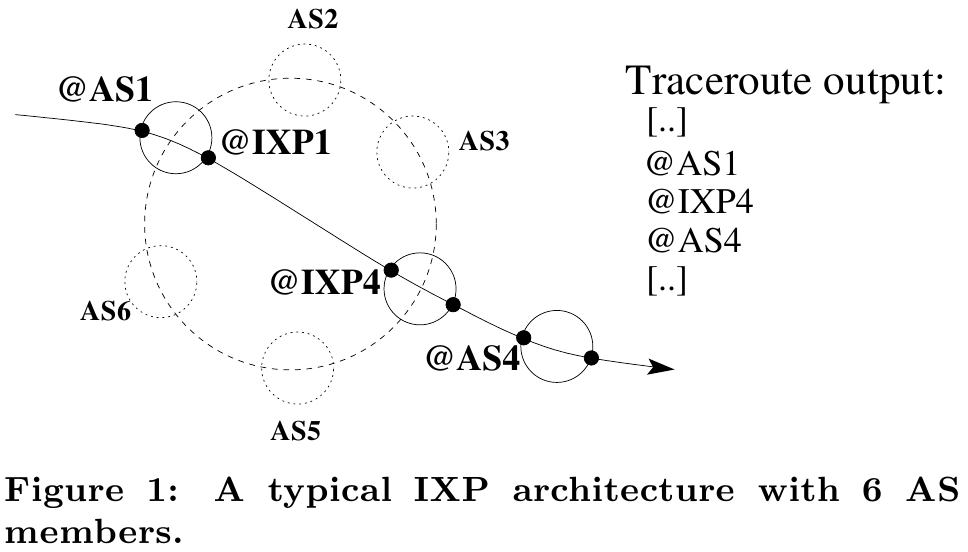
\includegraphics[width=1\textwidth]{augustin_ixp}
    \caption{Typische IXP Konfiguration mit 6 Mitgliedern - Entnommen aus~\cite{Augustin:2009:IM:1644893.1644934}}
    \label{fig:augustin_ixp}
  \end{center}
\end{figure}
Kritisch ist hierbei die Wahl des passenden traceroute Servers aber auch eine gewisse Vorsicht bei der Interpretation der Ergebnisse.
Die Tatsache, dass der Server im Netz des untersuchten ASes bedeutet nicht, dass aus Auftauchen oder Abwesenheit des oben beschriebenen Pfades mit Sicherheit auf die (Nicht-)Existenz des Peerings geschlossen werden kann.
Vor allem die Abwesenheit des Pfades ist trotz eines existierenden Peerings möglich.
IXPs vergeben an die teilnehmenden Router beispielsweise private IP-Adressen, auf die von außen nicht zugegriffen werden kann.

Weiterhin ist der Aufwand verglichen mit der Analyse vorhandener BGP dumps und updates verhältnismäßig hoch.
Es müssen aktiv Pakete gesendet und dabei timeouts abgewartet werden.
Außerdem ist die Gefahr, verfälschte Daten zu erhalten beim traceroute höher als bei der Analyse von BGP Daten, die zum Routing verwendet werden.

\subsubsection{Beitrag}
Augustin et~al. haben gezeigt, dass ein signifikanter Anteil der peer-to-peer Links alleine durch die Analyse von BGP dumps und updates nicht erfasst wird.
Weiterhin haben sie eine Liste von IXPs, deren Präfixen und Mitgliedern aufgebaut und traceroute Server in den ASen der Mitglieder identifiziert.
Diese Informationen wurden genutzt, um per gezieltem traceroute bisher nicht entdeckte Links an IXPs zu finden.
